\documentclass[9pt,xcolor=pdftex,dvipsnames,table]{beamer} 
\setbeamercolor{bgcolor}{fg=white,bg=blue!100}
\mode<presentation>
{
  \usetheme{Darmstadt}
 \setbeamertemplate{navigation symbols}{}
  \setbeamercovered{transparent}
  \setbeamertemplate{footline}
{\rightline{\insertframenumber/\inserttotalframenumber}}
}

\def\newblock{}

\newenvironment{changemargin}[2]{% 
  \begin{list}{}{% 
    \setlength{\topsep}{0pt}% 
    \setlength{\leftmargin}{#1}% 
    \setlength{\rightmargin}{#2}% 
    \setlength{\listparindent}{\parindent}% 
    \setlength{\itemindent}{\parindent}% 
    \setlength{\parsep}{\parskip}% 
  }% 
  \item[]}{\end{list}} 
  
\usepackage[english]{babel}
\usepackage{amsmath}
\usepackage{lipsum}
\usepackage[latin1]{inputenc}
\usepackage{times}
\usepackage[latin1]{inputenc}
\usepackage{tipa}
\usepackage{color}
\usepackage{booktabs}
\usepackage{colortbl}
\usepackage{movie15}
\usepackage{gb4e}
\usepackage{longtable}
\usepackage{pgf,pgfarrows,pgfnodes}
\usepackage{tikz} 
\usepackage{textpos}            % free image positioning 
\setlength{\TPVertModule}{1cm}  % unit for vertical positioning 
\setlength{\TPHorizModule}{1cm} % unit for horizontal positioning 

\definecolor{lightorange}{rgb}{1,0.75,.25}
\definecolor{lightred}{rgb}{1,0.25,.25}
\definecolor{lightblue}{rgb}{.25,.25,1.0}
\definecolor{lightgray}{rgb}{.75,.75,.75}

\usepackage[T1]{fontenc}

\title{How To Wreck a Nice Beach}
\author{Linguistics 409 $\cdot$ Computational Linguistics}
\date{}
\usepackage{gb4e}

\usepackage{natbib}
\bibliographystyle{apalike}

\makeatletter
\newcommand\textsubscript[1]{\@textsubscript{\selectfont#1}}
\def\@textsubscript#1{{\m@th\ensuremath{_{\mbox{\fontsize\sf@size\z@#1}}}}}
\newcommand\textbothscript[2]{%
  \@textbothscript{\selectfont#1}{\selectfont#2}}
\def\@textbothscript#1#2{%
  {\m@th\ensuremath{%
    ^{\mbox{\fontsize\sf@size\z@#1}}%
    _{\mbox{\fontsize\sf@size\z@#2}}}}}
\def\@super{^}\def\@sub{_}
\makeatother

\begin{document}
\definecolor{grey}{rgb}{1,0.6,.7}

\section{Automatic Speech Recognition}

\begin{frame}

	\titlepage
	\vspace{-1.5cm}
	\begin{center}
    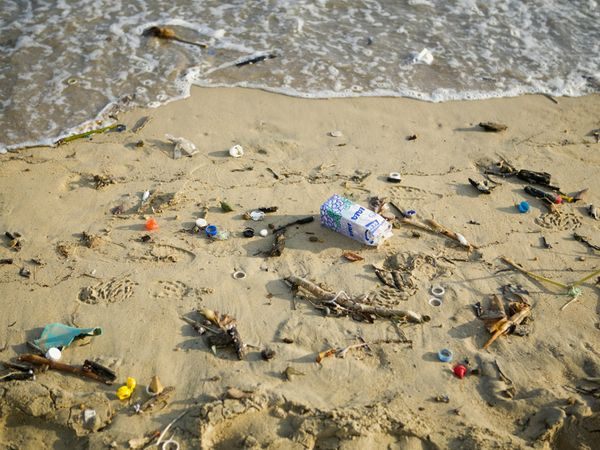
\includegraphics[scale=.4]{niceBeach.jpg}
	\end{center}
	
\end{frame}

\subsection{}
\begin{frame}{Alphabets}
    \setbeamercovered{invisible}

	\begin{itemize}
		\item To be precise, a string is a sequence of zero or more symbols drawn from a particular \emph{alphabet} $\Sigma$.
		\item We will refer to the special case of a null string, a string with zero symbols, with lowercase epsilon: {\large $\epsilon$}
		\item An alphabet can contain any unordered collection of unique symbols (a \textbf{set}).
		\item For example:
			\begin{itemize}
				\item $\Sigma_i = {a, b, c, d, e}$
				\item $\Sigma_j = {foo, bar, baz, qux}$ 
				\item ...
			\end{itemize}
	\end{itemize}
\end{frame}


\subsection{}
\begin{frame}{For next time:}
     \begin{block}{For next time:}
          \begin{enumerate}
     	  \item Assignment 1 will be posted tonight.\\
          \item There will be a short UNIX reading on OwlSpace for Wednesday.\\
          \item Please bring a computer if you have one!\\
          \item Wednesday: \textbf{Wrap up FSAs \& Start UNIX}
          \end{enumerate}
     \end{block}
\end{frame}



\end{document}


